\documentclass[t]{beamer}  % [t], [c], или [b] --- вертикальное выравнивание на слайдах (верх, центр, низ)
%\documentclass[handout]{beamer} % Раздаточный материал (на слайдах всё сразу)
%\documentclass[aspectratio=169]{beamer} % Соотношение сторон

%%% Работа с русским языком
\usepackage{cmap}					% поиск в PDF
\usepackage{mathtext} 				% русские буквы в формулах
\usepackage[T2A]{fontenc}			% кодировка
\usepackage[utf8]{inputenc}			% кодировка исходного текста
\usepackage[english,russian]{babel}	% локализация и переносы

%% Beamer по-русски
\newtheorem{rtheorem}{Теорема}
\newtheorem{rproof}{Доказательство}
\newtheorem{rexample}{Пример}

%%% Дополнительная работа с математикой
\usepackage{amsmath,amsfonts,amssymb,amsthm,mathtools} % AMS
\usepackage{icomma} % "Умная" запятая: $0,2$ --- число, $0, 2$ --- перечисление

%% Номера формул
%\mathtoolsset{showonlyrefs=true} % Показывать номера только у тех формул, на которые есть \eqref{} в тексте.
%\usepackage{leqno} % Нумерация формул слева

%% Свои команды
\DeclareMathOperator{\sgn}{\mathop{sgn}}

%% Перенос знаков в формулах (по Львовскому)
\newcommand*{\hm}[1]{#1\nobreak\discretionary{}
{\hbox{$\mathsurround=0pt #1$}}{}}

%%% Работа с картинками
\usepackage{graphicx}  % Для вставки рисунков
\graphicspath{{images/}{images2/}}  % папки с картинками
\setlength\fboxsep{3pt} % Отступ рамки \fbox{} от рисунка
\setlength\fboxrule{1pt} % Толщина линий рамки \fbox{}
\usepackage{wrapfig} % Обтекание рисунков текстом

%%% Работа с таблицами
\usepackage{array,tabularx,tabulary,booktabs} % Дополнительная работа с таблицами
\usepackage{longtable}  % Длинные таблицы
\usepackage{multirow} % Слияние строк в таблице

%%% Программирование
\usepackage{etoolbox} % логические операторы

%%% Другие пакеты
\usepackage{lastpage} % Узнать, сколько всего страниц в документе.
\usepackage{soul} % Модификаторы начертания
\usepackage{csquotes} % Еще инструменты для ссылок
%\usepackage[style=authoryear,maxcitenames=2,backend=biber,sorting=nty]{biblatex}
\usepackage{multicol} % Несколько колонок

%%% Картинки
\usepackage{tikz} % Работа с графикой
\usepackage{pgfplots}
\usepackage{pgfplotstable}

\title{Доклад на тему:}
\subtitle{Суффиксные деревья. Алгоритм Укконена}
\author{Валерий Буканов}
\date{\today}
\institute[СПбГУ]{Санкт-Петербургский государственный университет}

\begin{document}

\frame[plain]{\titlepage}	% Титульный слайд

\section{Оглавление}
\begin{frame}
	\frametitle{\insertsection}
	\begin{large}
		\begin{enumerate}
			\item Введение 
			\begin{enumerate}
				\item Немного истории
				\item Понятие суф. дерева
				%\item Некоторые примеры использования
			\end{enumerate}
			\item Построение суф. деревьев
			\begin{enumerate}
				\item Наивный подход
				\item Первые улучшения
				\item Финальная версия
				\item Оценка времени работы
			\end{enumerate}
			\item Итоги
			\begin{enumerate}
				%\item Минусы алгоритма
				%\item Нерешенные проблемы
				%\item Применения
				\item Ссылки и материалы
			\end{enumerate}
		\end{enumerate}
	\end{large}
\end{frame}


\section{Введение}
\subsection{История}
 
\begin{frame}[c]
	\frametitle{\insertsection} 
	\framesubtitle{\insertsubsection}
	
	\large \textbf{Суффиксное дерево} было создано Питером Вайнером в 1973 году. 	
	Первое название -- position tree. 
	
	> 92 тыс. цитирований в Google Scholar 
	
	Дональд Кнут назвал его \textbf{"Лучший алгоритм 1973 года"}.
	
	\pause
	Как Вы думаете в чем схожесть Вайнера и PSY?
	
	\pause 
	Они оба авторы одного хита
\end{frame}

\subsection{Основные понятия}

\begin{frame}[c]
	\frametitle{\insertsubsection}
    
    Пусть дан текст T = $t_{1}t_{2}$ \ldots $t_{n}$ и паттерн P = $p_{1}$ \ldots $p_{n}$
    
    \pause
    \begin{block}{Определение}
    	 \textbf{Суффиксное дерево} (suffix tree ST) -- сжатый бор, построенный на всех суффиксах строки T\$.
    \end{block}
    \pause
    
    Будем хранить на ребрах вместо подстрок их индексы в исходной строке $T[i....j]$ 
    
    \pause
   	\textbf{Таким образом:} \pause
   	
    \begin{itemize}
        \item<1-> Ни один суффикс в ST не может полностью лежать в другом \pause
        \item<2-> Расходуется $O(n)$ памяти
    \end{itemize}

\end{frame}

\section{Построение суффиксного дерева}
\subsection{Наивный подход}
\begin{frame}
	\frametitle{\insertsection}
	\framesubtitle{\insertsubsection}
	\begin{block}{Online подход:}
		Будем строить суффиксное дерево итеративно, добавляя на каждом шаге по одному символу текста T. То есть будем строить ST для всех префиксов текста T.
		
		\pause
		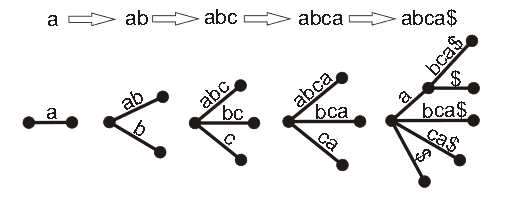
\includegraphics[width=\linewidth]{Example1}
	\end{block}	

\end{frame}

\begin{frame}
	\begin{block}{Псевдокод}
		for i = 1 .. n
		
		\qquad for j = 1 .. i
				
		\qquad \qquad treeExtend(s[j..i]) 
	\end{block}
	
	\pause
	Какова его асимптотика? \pause
	O($n^{3}$) \pause
	
	А зачем брать по одному символу? Нельзя ли брать сразу весь суффикс? \pause
	
	Можно, но это уже \href{http://wind.in.tum.de/seminare/textalgo/WS0203/Izamski.pdf}{ \textbf{совсем другая история...}}
	
\end{frame}

\begin{frame}{Виды продлений}
	\begin{itemize}
		\pause
		\item {\textbf{Продление листа.} Суффикс $s[k...i-1]$ заканчивается в листе. Добавим $s_{i}$ в конец подстроки, которая лежит на ребре, ведущем в лист.}
		
		\pause
		\item \textbf{Ответвление}
		\begin{itemize}
			\pause
			\item{ Суффикс $s[k...i-1]$ заканчивается в вершине (не листе), из которой нет пути по символу $s_{i}$. Создаем новый лист и на ребре пишем символ $s_{i}$.}
			
			\pause
			\item {Суффикс $s[k...i-1]$ заканчивается на ребре с путевой меткой $s[L...R]$ в позиции p - 1 и $s_{p} \neq  s_{i}$. 
				
				Разобьем ребро новой вершиной v на $s[L...p-1]$ и $s[p...R]$. Подвесим к вершине v нового ребенка с дугой, помеченной символом $s_{i}$. } 
			
		\end{itemize}
		\pause
		\item {\textbf{Ничего не делаем} Для суффикса $s[k...i-1]$ уже есть путь по символу $s_{i}$.} 
	\end{itemize}
\end{frame}

\subsection{Первые улучшения}
\begin{frame}
	\frametitle{\insertsubsection}
	
	\begin{block}{Определения}
		\textbf{Неявное суффиксное дерево} (implicit suffix tree IST) -- ST строки T без \$.
	\end{block}
	\pause
	
	\textbf{i-ая фаза алгоритма} -- продолжение всех суффиксов символом $t_{i}$.
	\pause
	
	Погрузимся в теорию...
\end{frame}

\subsection{Необходимые теоремы}
\begin{frame}
	\frametitle{\insertsubsection}
	
	Количество листьев в сжатом суффиксном дереве $O(n)$
	
	\pause
	\begin{rtheorem}
		\textbf{Количество внутренних вершин в сжатом суффиксном дереве меньше количества листьев}
	\end{rtheorem}
	\pause
	\begin{rproof}
		\begin{itemize}
			\pause
			\item индукция по n (количество вершин в дереве) \pause
			\item База n = 2: очевидно \pause
			\item Рассмотрим дерево на n + 1 вершине и найдем вершину, которая имеет не менее двух детей-листьев. \pause
			\item Если у этой вершины > 2 детей, отрежем одного и применим и.п.
			\pause
			\item Если у нее ровно 2 ребенка, отрежем обоих и также применим и.п. 
		\end{itemize}
	\end{rproof}
\end{frame}


\subsection{Первые улучшения}
\begin{frame}
	\frametitle{\insertsubsection}
	\pause
	Как же нам ускорять построение дерева?
	
	\pause
	Давайте использовать вспомогательные данные
	\pause
	
	\begin{block}{Определение}
			Пусть $x\alpha$ обозначает произвольную строку, где x -- ее первый символ, а $\alpha$ -- оставшаяся подстрока (возможно пустая). Если для внутренней вершины v с путевой меткой $x\alpha$ существует другая вершина sl(v) с путевой меткой $\alpha$, то ссылка из v в sl(v) называется \textbf{суффиксной ссылкой} (suffix link).
	\end{block}
	
	
\end{frame}

\begin{frame}
	\frametitle{\insertsubsection}
	\begin{block}{Лемма}
		$\forall$ внутренней вершины v $\exists$ суффиксная ссылка ведущая в какую-то внутреннюю вершину u. 
	\end{block}
	
	\pause
	\begin{rproof}
		Рассмотрим внутреннюю вершину v с путевой меткой $s[j...i]$. \pause
		 Так как эта вершина внутренняя, её путевая метка ветвится справа в исходной строке. \pause Тогда подстрока $s[j+1...i]$ тоже ветвится справа в исходной строке, и ей соответствует некоторая внутренняя вершина u. По определению суффиксная ссылка вершины v ведёт в u.
	\end{rproof}
\end{frame}

\begin{frame}
	\frametitle{\insertsubsection}
	
	\textbf{Задача:} научится эффективно переходить между суффиксами в фазах алгоритма
	\pause
	
	\begin{block}{Использование суф. ссылок}
		Пусть был продлен суффикс $s[j...i-1]$ до суффикса $s[j...i]$. Теперь надо продлить суффикс $s[j+1...i-1]$.
		
		Как быстро найти этот суффикс? \pause
		Пройдем вверх по дереву до ближайшей внутренней вершины v, перейдем по ее суффиксной ссылке в некоторую вершину u и спустимся по ребрам до нужного суффикса.
	\end{block}
	
	\pause Слишком \pause много \pause буков. \pause
	Обратимся к картинке
\end{frame}

\begin{frame}	
	\frametitle{\insertsubsection}
	
	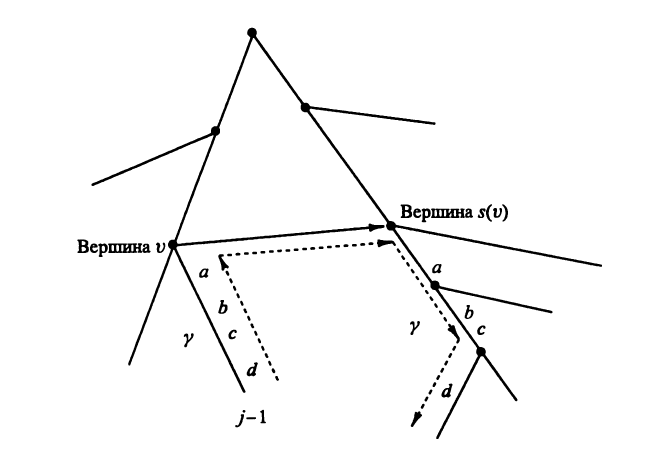
\includegraphics[width=\linewidth]{SuffixLink}
	
	А почему это быстро? \pause 
	Давайте узнаем
\end{frame}

\subsection{Обоснования улучшений}
\begin{frame}[shrink=12]	
	\frametitle{\insertsubsection}
	
	\textbf{Глубина вершины} -- количество ребер на пути от корня до этой вершины.
	
	\begin{block}{Лемма 1}
		При переходе по суффиксной ссылке глубина уменьшается не более чем на 1.
	\end{block}
	
	\begin{block}{Лемма 2}
		Число переходов по ребрам внутри фазы i равно $O(i)$.
	\end{block}
	\begin{rproof}
		\begin{itemize}
			\pause
			\item Проход вверх по ребру уменьшает глубину на 1
			\pause
			\item Проход по суффиксной ссылке уменьшает глубину не более чем на 1
			\pause
			\item Поэтому за фазу i совершается не более 2i переходов вверх
			\pause
			\item Заметим также, что в одной фазе начальная глубина меньше конечной, так как длины суффиксов уменьшаются
			\pause
			\item Следовательно вниз мы пошли тоже не более 2i раз
		\end{itemize}
	\end{rproof}

	\pause
	Поскольку всего n фаз и на каждой мы делаем $O(n)$ переходов, мы получили асимптотику O($n^{2}$)
\end{frame}

\subsection{Финальная версия}
\begin{frame}	
	\frametitle{\insertsubsection}

	\textbf{Ключевые леммы}
	\pause
	
	\begin{block}{Лемма (Стал листом — листом и останешься):}
		Если в какой-то момент был создан лист с меткой i, он останется листом во всех последовательных деревьях, созданных алгоритмом.
	\end{block}
	\pause
	\begin{rproof}
		\begin{itemize}	
			\item Внимательно прочитав правила продления, мы увидим, что у нас нет правила продолжения листового ребра дальше текущего листа.
			\pause
			\item Если есть лист с суффиксом i, то правило 1 будет применяться для продолжения i на всех остальных фазах. 
		\end{itemize}
	\end{rproof}	
\end{frame}

\begin{frame}	
	\frametitle{\insertsubsection}
	
	\textbf{Ключевые леммы}
		
	\begin{block}{Лемма (правило 3 заканчивает дело):}
		Если правило продления 3 применяется в продолжении суффикса, начинающегося в позиции $j$, это же правило будет применяться ко всем остальным суффиксам $(j+1...i)$ до конца фазы.
	\end{block}
	\pause
	\begin{rproof}
		\begin{itemize}
			\pause
			\item При продолжении по правилу 3 путь помеченный суффиксом $s[j...i-1]$ должен продолжаться символом $s_{i}$. 
			\pause
			\item Точно так же продолжаются все остальные пути помеченные $s[j+1...i-1], s[j+2...i-1]$ и тд. 
		\end{itemize}
	\end{rproof}
\end{frame}

\begin{frame}
	\frametitle{\insertsubsection}
	\begin{block}{Алгоритм}
		\begin{itemize}
			\item Храним в листьях переменную x и неявно продлеваем их за $O(1)$.
			\pause
			\item Алгоритм явно работает с суффиксами в диапазоне 
			\\от $j^{*}$ до $k$, $k \leq i$.
			\pause
			\item Действительно, если суффикс $s[j...i-2]$ был продлён до суффикса $s[j...i-1]$ на прошлой фазе по правилу 1, то он и дальше будет продлеваться по правилу 1.
			\pause
			\item Если он был продлён по правилу 2, то была создана новая листовая вершина, значит, на текущей фазе i этот суффикс будет продлён по листу.
			\pause
			\item Следовательно после применения правила 3 на суффиксе $s[k...i]$ текущую фазу можно завершить, а следующую начать с $j^{*} = k - 1$.
		\end{itemize}
	\end{block}
\end{frame}

\begin{frame}
	\frametitle{Линейная оценка}
	Пусть cur это наша текущая вершина
	
	\begin{block}{Псевдокод}
		\pause
		\begin{enumerate}
			\item\color[RGB]{0,0, 255}for \color[RGB]{0,0,0} c in s:
			
			\pause
			\item \qquad \color[RGB]{0,0, 255}while \color[RGB]{0,0,0}True:
			
			\pause
			\item \qquad\qquad \textbf{if} есть переход из cur по c:
			
			\pause
			\item \qquad\qquad\qquad cur = переход из cur по с 
			
			\pause
			\item \qquad\qquad\qquad \textbf{break}
			
			\pause
			\item \qquad\qquad \textbf{else}:
			
			\pause
			\item \qquad\qquad\qquad Сделать переход из cur по c
			
			\pause
			\item \qquad\qquad\qquad Дописываем туда все символы	//лист
			
			\pause
			\item \qquad\qquad\qquad cur = переход из cur по суф. ссылке 
				
			\pause	
			\item \qquad\qquad\qquad prev.sufflink = cur 		
		\end{enumerate}
	\end{block}

	\pause
	Суммарное время работы алгоритма $O(n)$
\end{frame}

\begin{frame}
	\frametitle{Источники}
	
	\begin{itemize}
		\item Дэн Гасфилд — Строки, деревья и последовательности в алгоритмах: Информатика и вычислительная биология — СПб.: Невский Диалект; БХВ-Петербург, 2003. — 654 с: ил.
		
		\item \href{http://yury.name/internet/01ianote.pdf}{\textbf{Коспект Юрия Лифшица}}
		
		\item Викиконспекты
		
		\item \href{https://www.youtube.com/watch?v=LNBs3xZMGLc}{\textbf{Видеолекции Павла Маврина}}
		
		\item \href{https://habr.com/ru/post/111675/}{\textbf{Habr}}
	\end{itemize}	
\end{frame}
\end{document}